\subsection{线段分析}
平面图形中各线段(直线或圆弧)的定位尺寸数量直接影响绘图先后顺序,而定形尺寸是不可缺少的。根据定形尺寸和定位尺寸的数量可将线段分类三类。

\subsubsection{已知线段}
已知线段是有足够的定位尺寸和定形尺寸,不需要利用与其它线段的连接关系即可直接画出的直线或圆弧。图\ref{fig:biaozu2}所示的即为图\ref{fig:biaozu}的已知线段。

\subsubsection{中间线段} 

中间线段是缺少一个定位尺寸,需要通过与其相邻一边的图线的连接关系,才能够作出的直线或圆弧。图\ref{fig:biaozu3}是在图\ref{fig:biaozu2}的基础上绘出所有的中间线段。
\subsubsection{连接线段} 

连接线段是缺少两个定位尺寸,需要通过与两边相邻的图形的连接关系,才能够绘出的直线或圆弧。图\ref{fig:biaozu4}是在图\ref{fig:biaozu3}的基础上绘制所有的连接线段。

\begin{figure}[htbp]
\centering
\subfloat[已知线段]{\label{fig:biaozu2}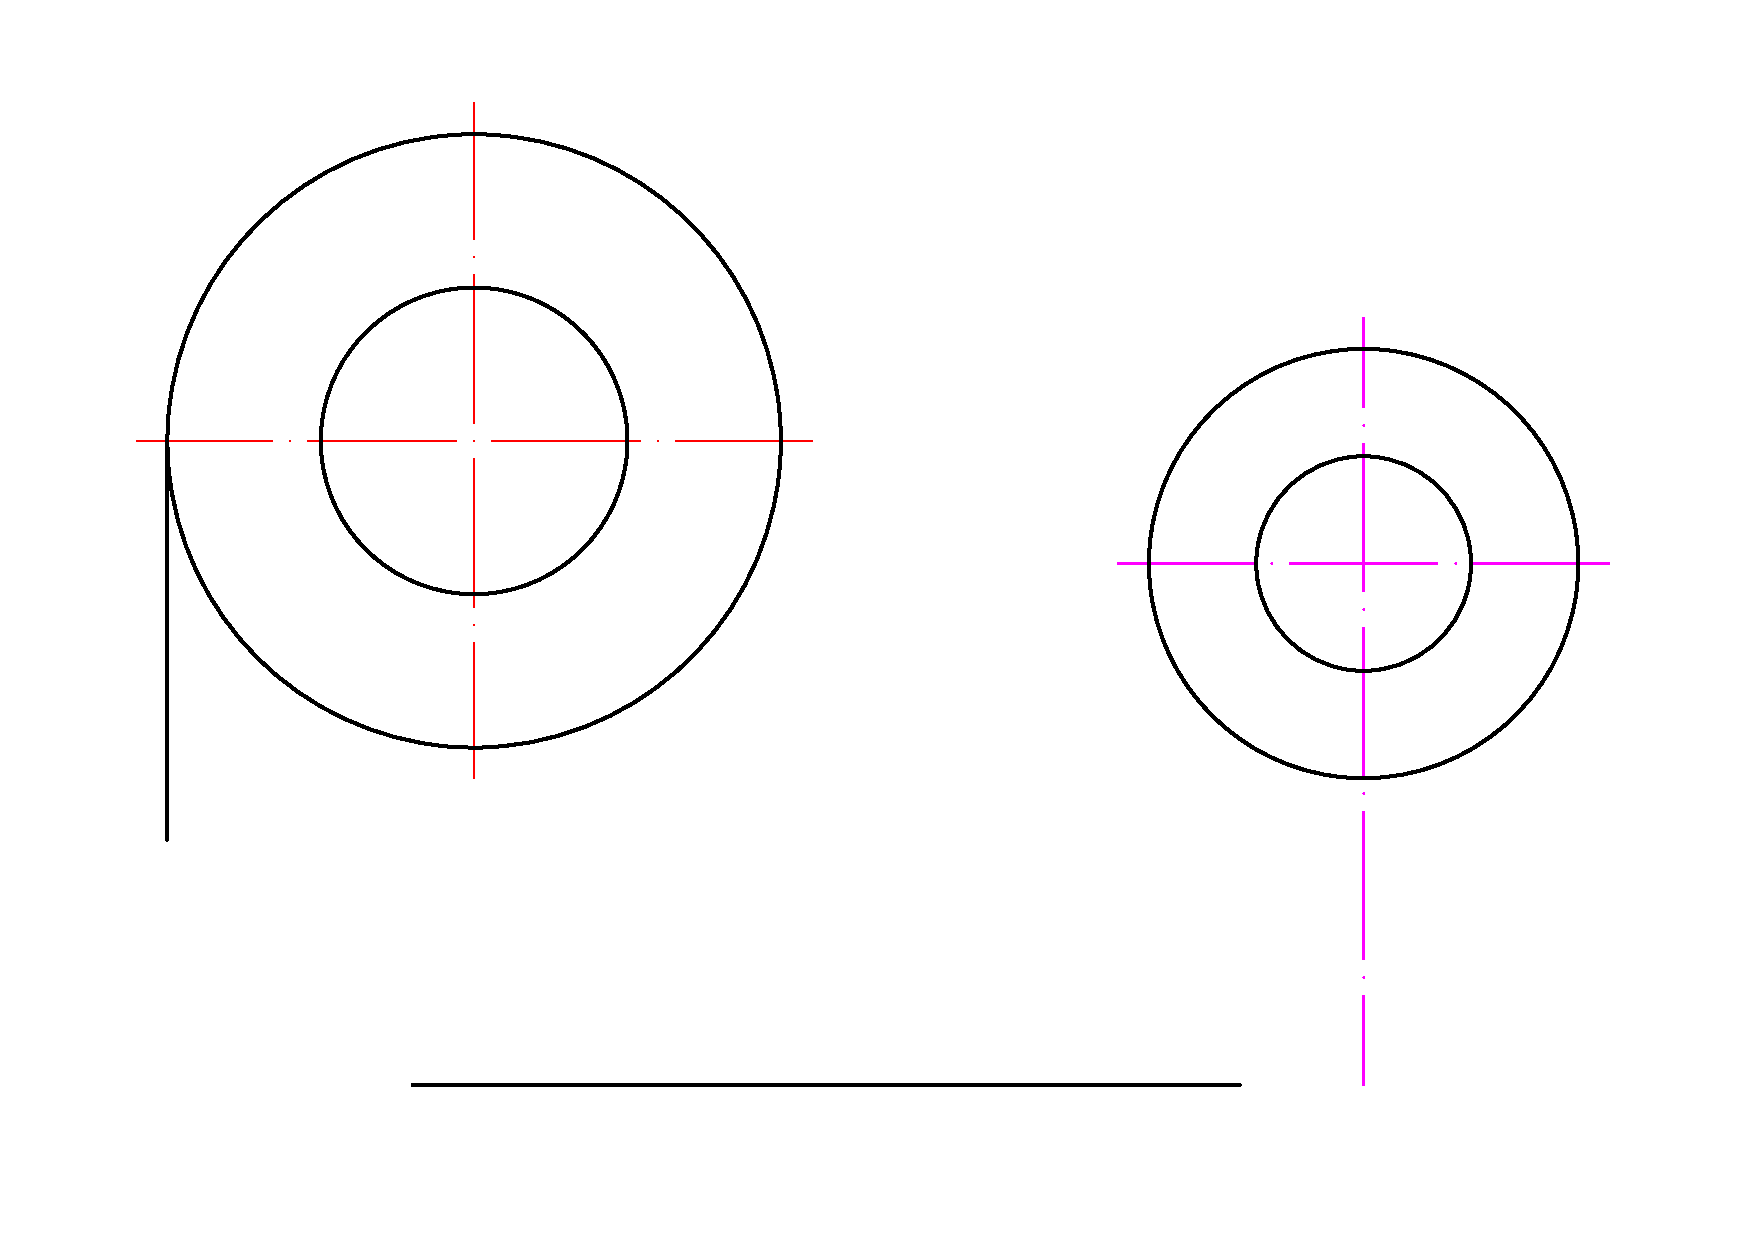
\includegraphics[scale=0.15]{biaozu2.pdf}}\hspace{20pt}
\subfloat[中间线段]{\label{fig:biaozu3}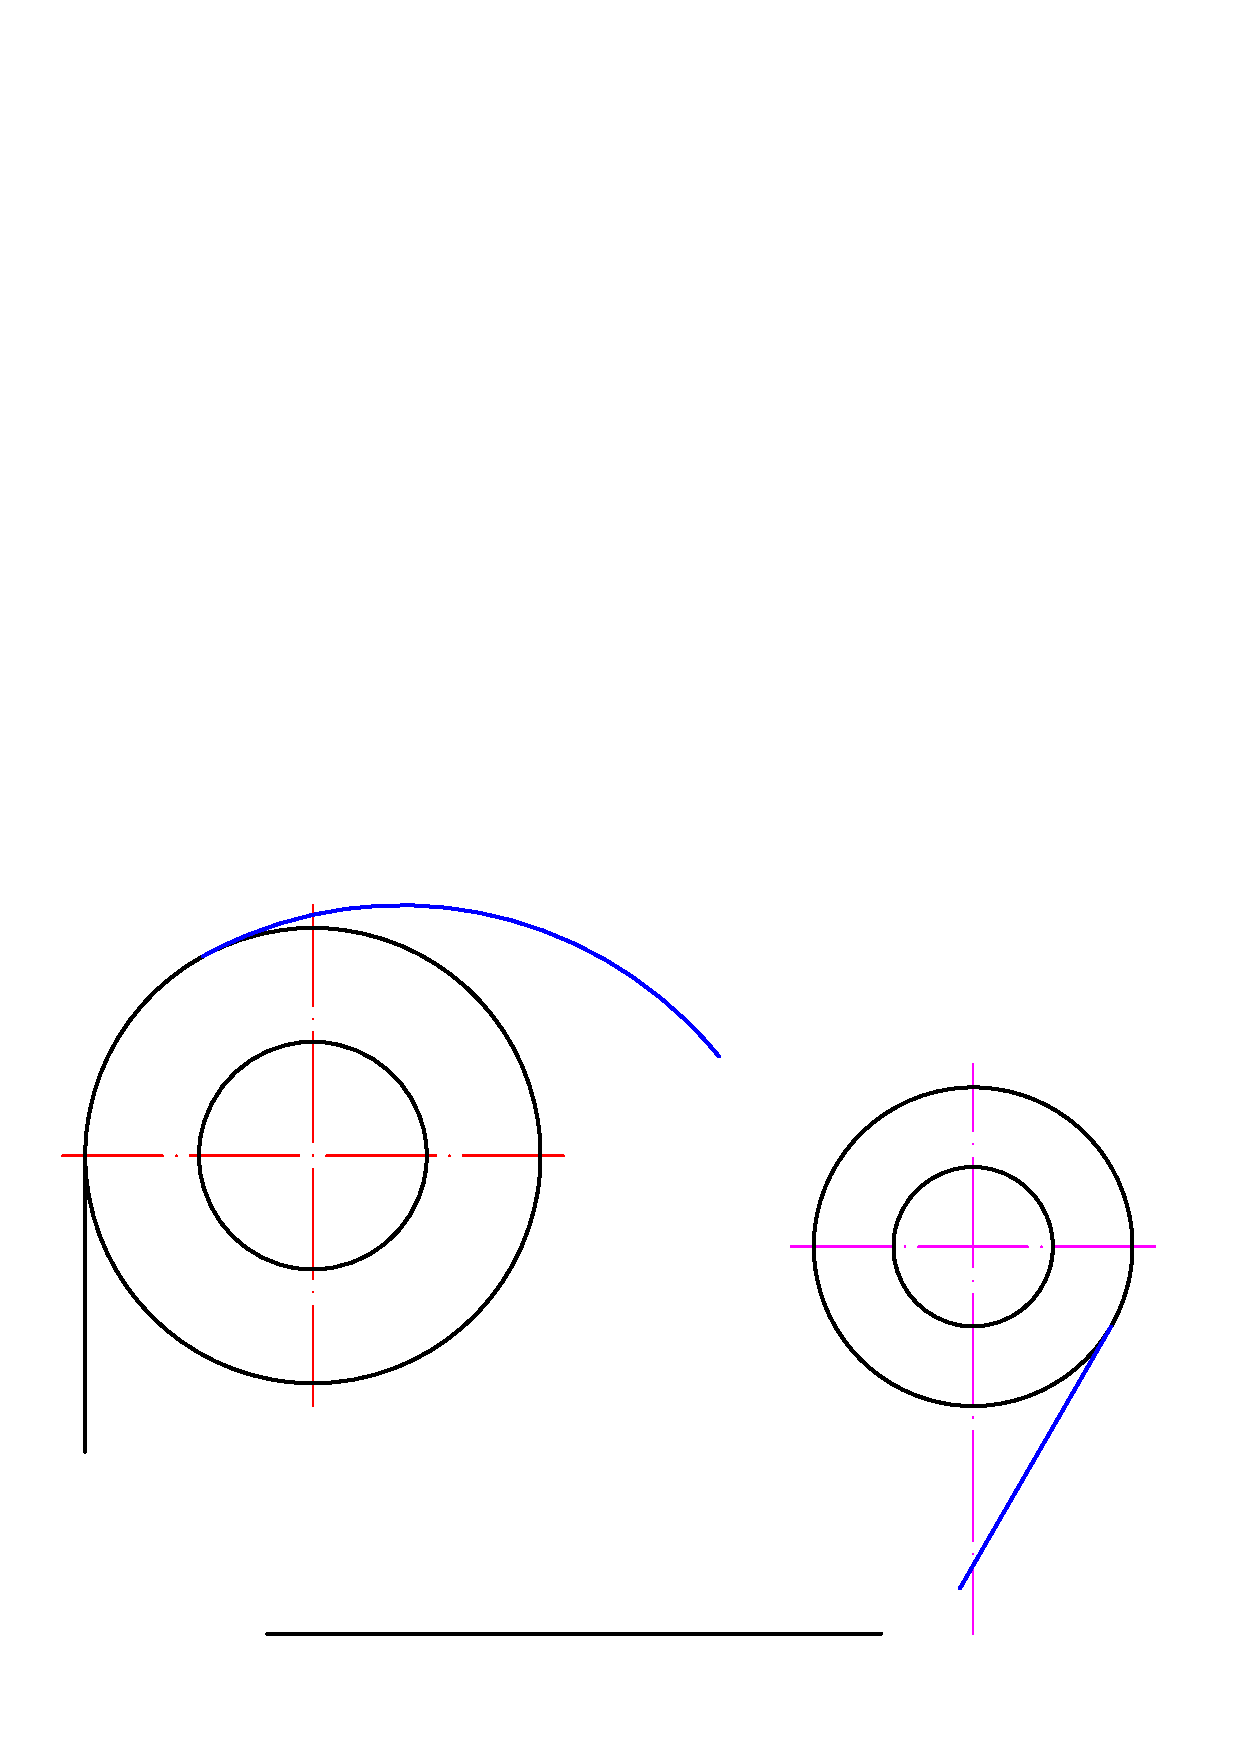
\includegraphics[scale=0.2]{biaozu3.pdf}}\hspace{20pt}
\subfloat[连接线段]{\label{fig:biaozu4}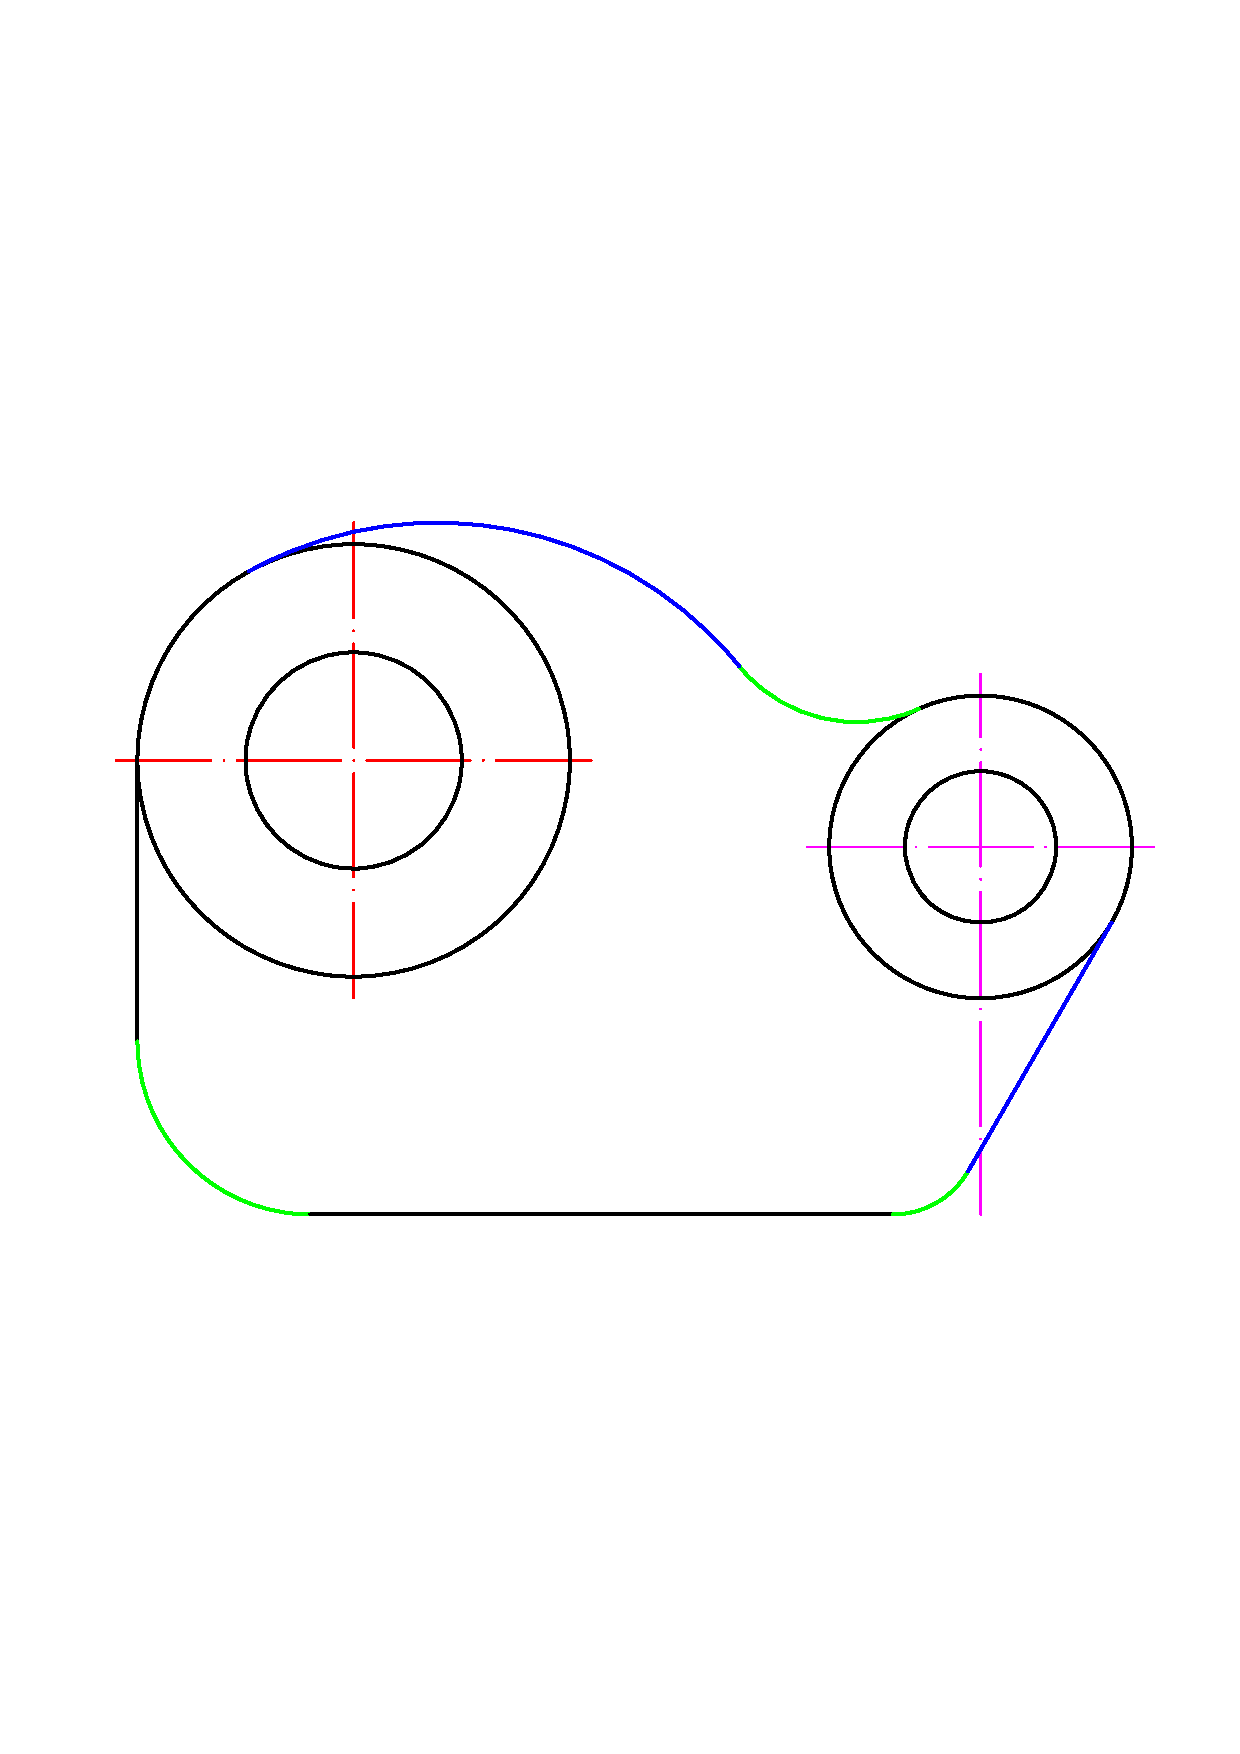
\includegraphics[scale=0.2]{biaozu4.pdf}}
\caption{平面图形中的线段分析}
\end{figure}
